\section{Background and Motivation}

  In this section, we first introduce the background of batch stream processing and stragglers. Then we deep into the problems existing in traditional straggler mitigation strategies when processing short stream jobs. We also briefly analyze the characteristics of recurring batch stream jobs. Finally, we outline the challenges in pre-scheduling straggler mitigation.

\subsection{Background}

  Batch Stream Processing System treats a streaming computation as a series of deterministic batch computations on small time intervals \cite{Zaharia2013}. As shown in Figure 1, Batch Stream Processing System (1) receives input data and divides continuous data stream into a series of small batches according to batch interval (a time granularity which is set according to application's response time), (2) when each batch interval arrives, batch jobs are generated for each batch, (3) these jobs would be repeatedly submitted to batch processing engine such as MapReduce or Spark and are re-run periodically to execute with distributed fault tolerance, data locality scheduling and load balancing provided by batch framework automatically. Latency sensitive, micro jobs/tiny tasks and recurring jobs are three dominant characteristics of these systems.
  \begin{figure}[htbp]
    \centering
    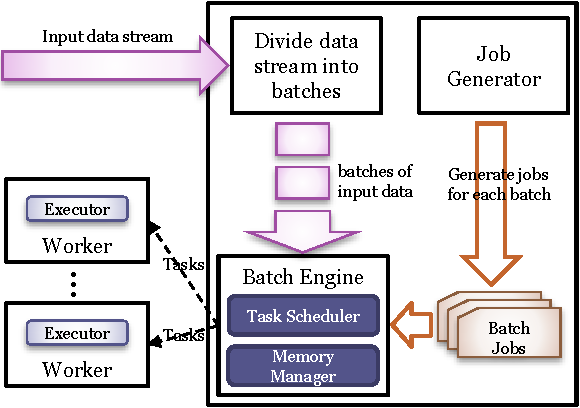
\includegraphics[width=0.34\textwidth]{FigureBatchStream}
    \caption{Principles of Batch Stream Processing System}\label{Fig. 1:}
  \end{figure}

  Stragglers have been a primary performance issue for batch stream processing system. Because the whole job must wait for the slowest task. These stragglers cause unproductive wait time for all the others, delaying job completion. Stragglers especially impact short batch stream jobs. On the one hand, short batch stream jobs are more latency-sensitive and require short response time. On the other hand, short batch stream jobs consist of just a few tasks. Such jobs typically get to run all their tasks at less waves. So, if one task straggles, the whole job is significantly delayed. Beyond these, if a job is so severely affected by stragglers that its completion time exceeds one batch interval, it will delay the next job's submission and execution. Stragglers can occur for many reasons, including hardware heterogeneity \cite{Reiss2012}, data skew \cite{Kwon2012}, hardware failures \cite{Ananthanarayanan2010}, energy efficient \cite{Cheng2015}, resource contention and various OS effects.

\subsection{Problem Analysis}

  Existing methods to straggler mitigation are post-scheduling methods. They fall short in multiple ways. Reactive approaches whether or not based on replication react after tasks have already slowed down. Proactive approaches which use replication incur extra resources. Proactive approaches without replication still take hysteretic actions after some nodes show stragglers' indications and need to migrate data at runtime. For short batch stream jobs, these approaches spend much reactive time to eliminate stragglers and cause other nodes to be idle over a period of time, wasting cluster computing cycles. In the following, we analyze four representative approaches. They are Speculative execution, SkewTune, Dolly and Wrangler on behalf of reactive approach with replication, reactive approach without replication, proactive approach with replication and proactive approach without replication respectively.
  \begin{figure*}[htbp]
    \centering
    \subfloat[Speculative Execution]{%
      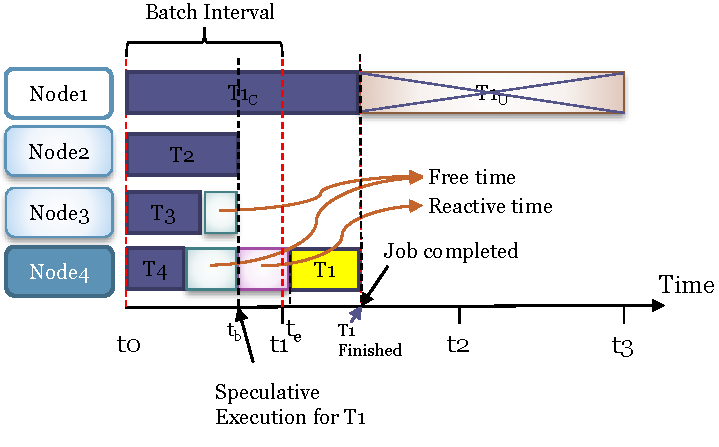
\includegraphics[width=0.42\textwidth]{Figure5a}
    }
    \subfloat[SkewTune]{%
      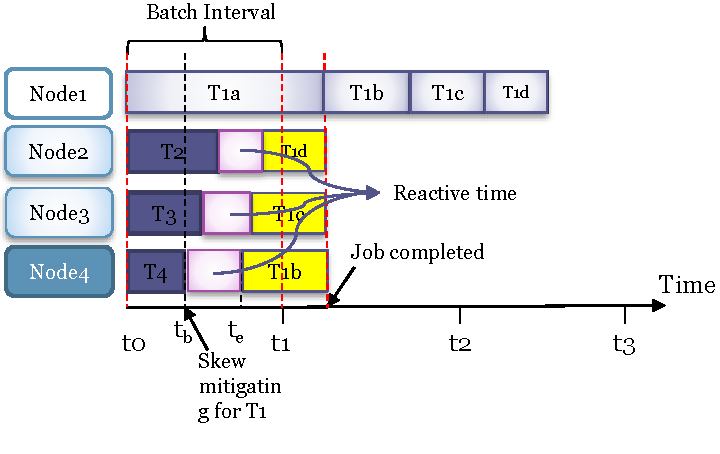
\includegraphics[width=0.42\textwidth]{Figure5b}
    }\hfill
    \subfloat[Dolly]{%
      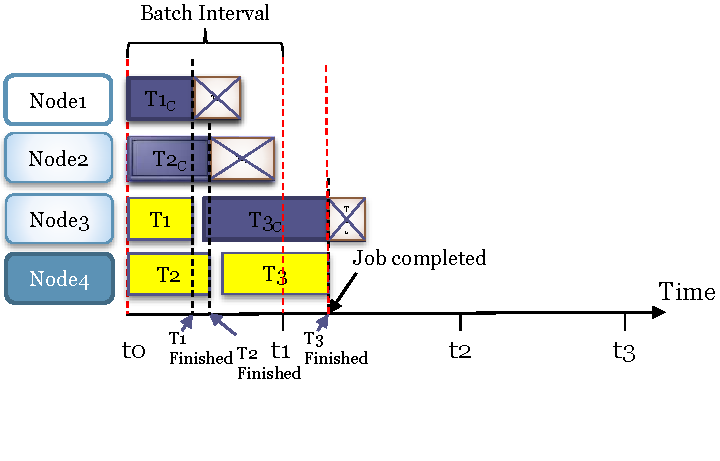
\includegraphics[width=0.42\textwidth]{Figure5c}
    }
    \subfloat[Wrangler]{%
      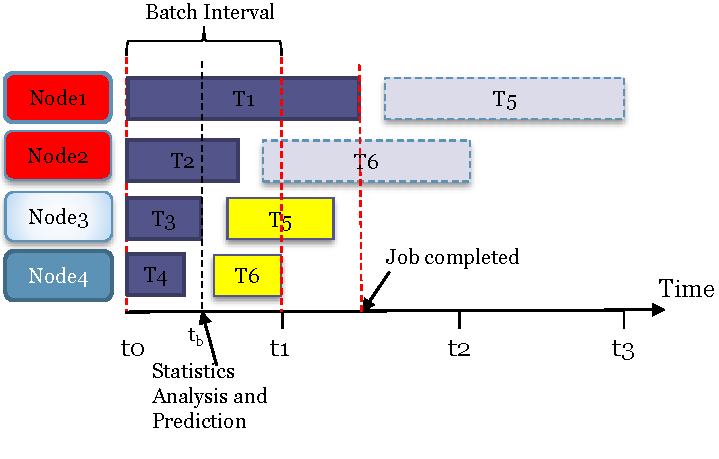
\includegraphics[width=0.42\textwidth]{Figure5d}
    }\hfill
    \caption{Straggler mitigation under different strategies}
    \label{Fig. 2:}
  \end{figure*}

  Reactive approaches rely on a wait-speculate-re-execute mechanism. Speculative execution \cite{Dean2004} is a widely used reactive approach with replication for straggler mitigation. Speculative execution marks slow running tasks as stragglers and reacts by re-launching multiple copies of them. As soon as one of these copies finishes execution, the rest are killed. Taking Fig. 2(a) as an example, at $t_b$, T1 is marked as stragglers. Then speculative execution launches a copy of T1 on node4. It migrates data block of Task T1 to node4 and starts executing at $t_e$. As we can see, this approach incurs long reactive time and free time for other nodes. It becomes inefficient for short batch stream jobs in two aspects. On one hand, a task must run for a significant amount of time before it can be identified as a straggler. By this time, other tasks of that job have made considerable progress already. On the other hand, the reactive procedure is time-consuming in terms of short stream job. A short stream job of several seconds response time is not allowed to spend several seconds on doing speculating and migrating. LATE \cite{Zaharia2008} is an enhanced version of speculative execution using a notion of progress scores, but is still a wait-speculate-re-execute mechanism.

  SkewTune \cite{Kwon2012} is still a reactive approach but without replication. As soon as one node has an available slot, SkewTune begins to detect data skew and identify stragglers according to each task's remaining time. As shown in Fig. 2(b), when task T4 is completed at $t_b$, SkewTune's detection is triggered. Node1 is identified as straggler. T1 is selected to do skew mitigation due to its long remaining progress. Then SkewTune scans T1's remaining input data and repartitions T1's remaining work into T1b, T1c and T1d. Finally, T1b, T1c and T1d are scheduled and migrated to remote faster nodes node4, node3 and node2 respectively. From $t_b$ to $t_e$, this procedure incurs approximately 2 seconds overhead for a task with 2MB's input data. This overhead grows linearly with the size of the task's input data. However, this overhead is intolerant for short stream jobs which must be completed in several seconds or sub-seconds. Furthermore, before SkewTune begins working, task T1 has already slowed down. Although SkewTune avoids replicating tasks but is still a wait-and-speculate mechanism.

  Dolly \cite{Ananthanarayanan2013} is a proactive strategy by full cloning of small jobs. Dolly launches multiple clones of every task of a job and only use the result of the clone that finishes first. As shown in Fig. 2(c), Dolly launches two clones of Task T1 and Task T2 in node1,3 and node2,4 respectively. After T1 and T2 complete, Dolly schedules T3 and also launches two clones of Task T3 in node3,4. Dolly gets the results from which finishes first such as Task T1 in node3 and kills other uncompleted clones such as Task T1 in node1. This not only amounts to wastage of resources, but also delays successor tasks.

  Unlike Dolly, Wrangler \cite{Yadwadkar2014} is a proactive strategy without replication. It predicts stragglers using an interpretable linear modeling technique based on cluster resource usage counters and uses these predictions to inform scheduling decisions. For example, in Fig. 2(d), Wrangler analyzes statistics and make predictions about stragglers at $t_b$. Node1 and node2 are identified as stragglers. Then Wrangler schedules and migrates T5 in node1, T6 in node2 onto node3 and node4 respectively. Although this approach can avoid successor possible stragglers, it remains taking hysteretic actions for short batch stream jobs. Because short batch stream jobs always consist of a few tasks and get to run at once. Furthermore, Wrangler can't act until some nodes show some indications of stragglers(eg. high cpu utilization, heavy memory access, network congestion). It also need to migrate data block at runtime regardless of data locality.

  In summary, existing post-scheduling approaches fall short when processing short stream jobs. Reactive approaches act after stragglers have occurred. At that time, tasks have already slowed down. Replication-based proactive approaches incur extra resource and increase 2x load of the cluster. Proactive approaches without replication also take hysteretic actions after some nodes show some indications of stragglers. We need to design a pre-scheduling straggler mitigation strategy for short batch stream jobs which can eliminate stragglers as early as possible.

\subsection{Recurring Batch Stream Jobs}

  Batch stream jobs are typically recurring with stable code and data properties. Many characteristics such as application logic, stragglers, resource utilization, scheduling and other operations present statistically similar to the previous execution when running on newer data of the same stream \cite{Agarwal}. Figure 3(a) plots the average difference between statistics collected at the same location across different batches' jobs. We ran WordCount in our testbed and picked all the jobs from 50 batches, while the batch repeated in 2s' batch interval. The overall statistics are similar across jobs, the ratio stdev/mean is less than 0.2 for 70\% of the locations. Figure 3(b) shows the resource utilization. These jobs cost almost the same amount of computational resources.
  \begin{figure}[htbp]
    \centering
    \subfloat[Data Properties]{%
      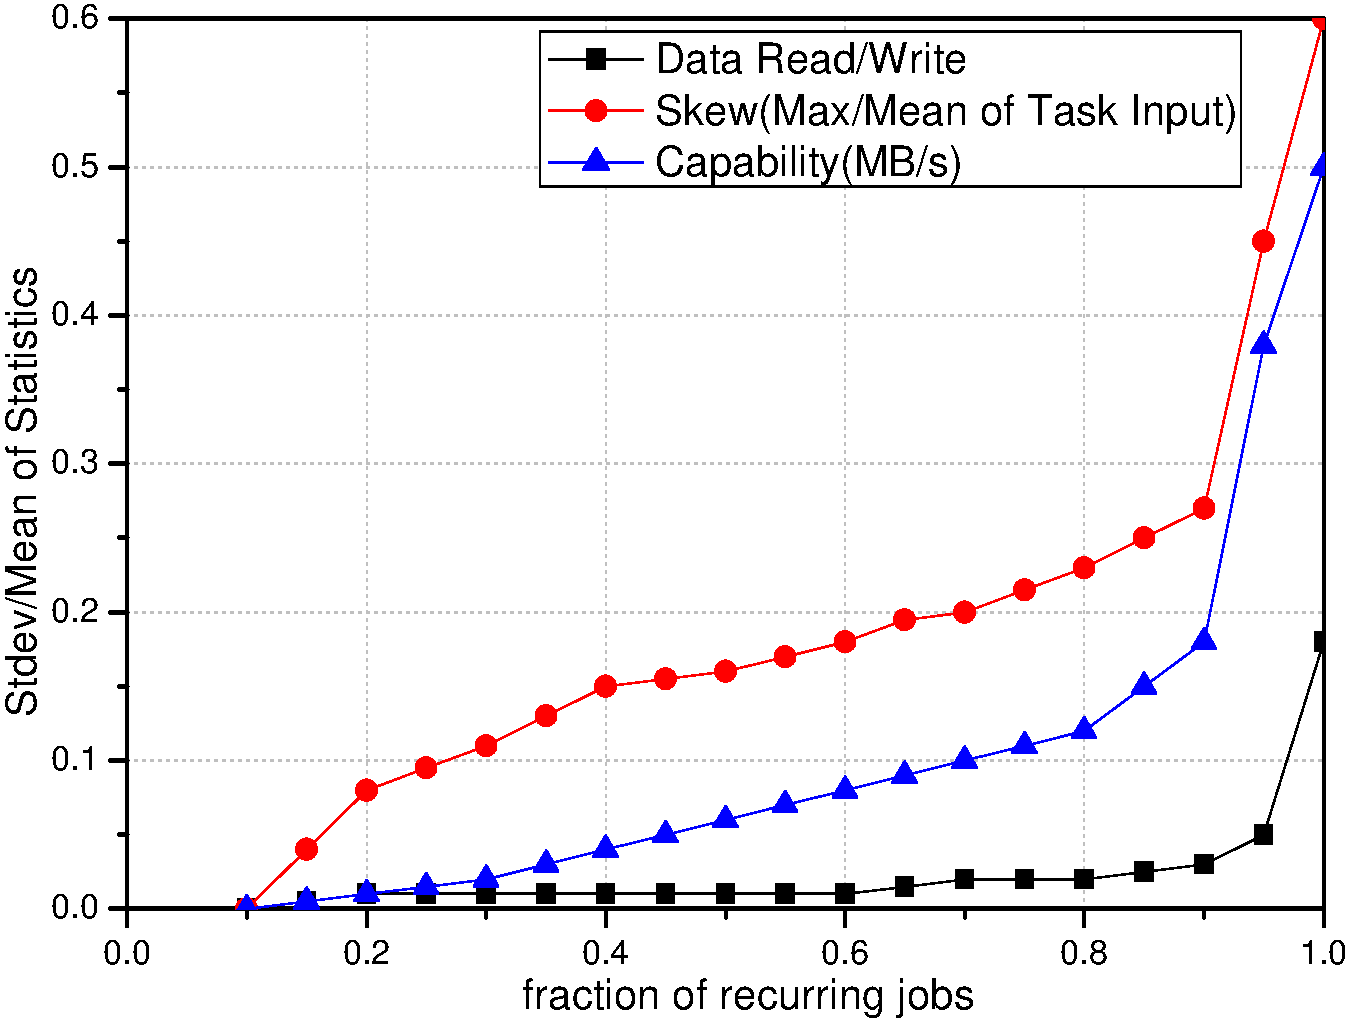
\includegraphics[width=0.235\textwidth]{Figure3}
    }
    \subfloat[Resource Utilization]{%
      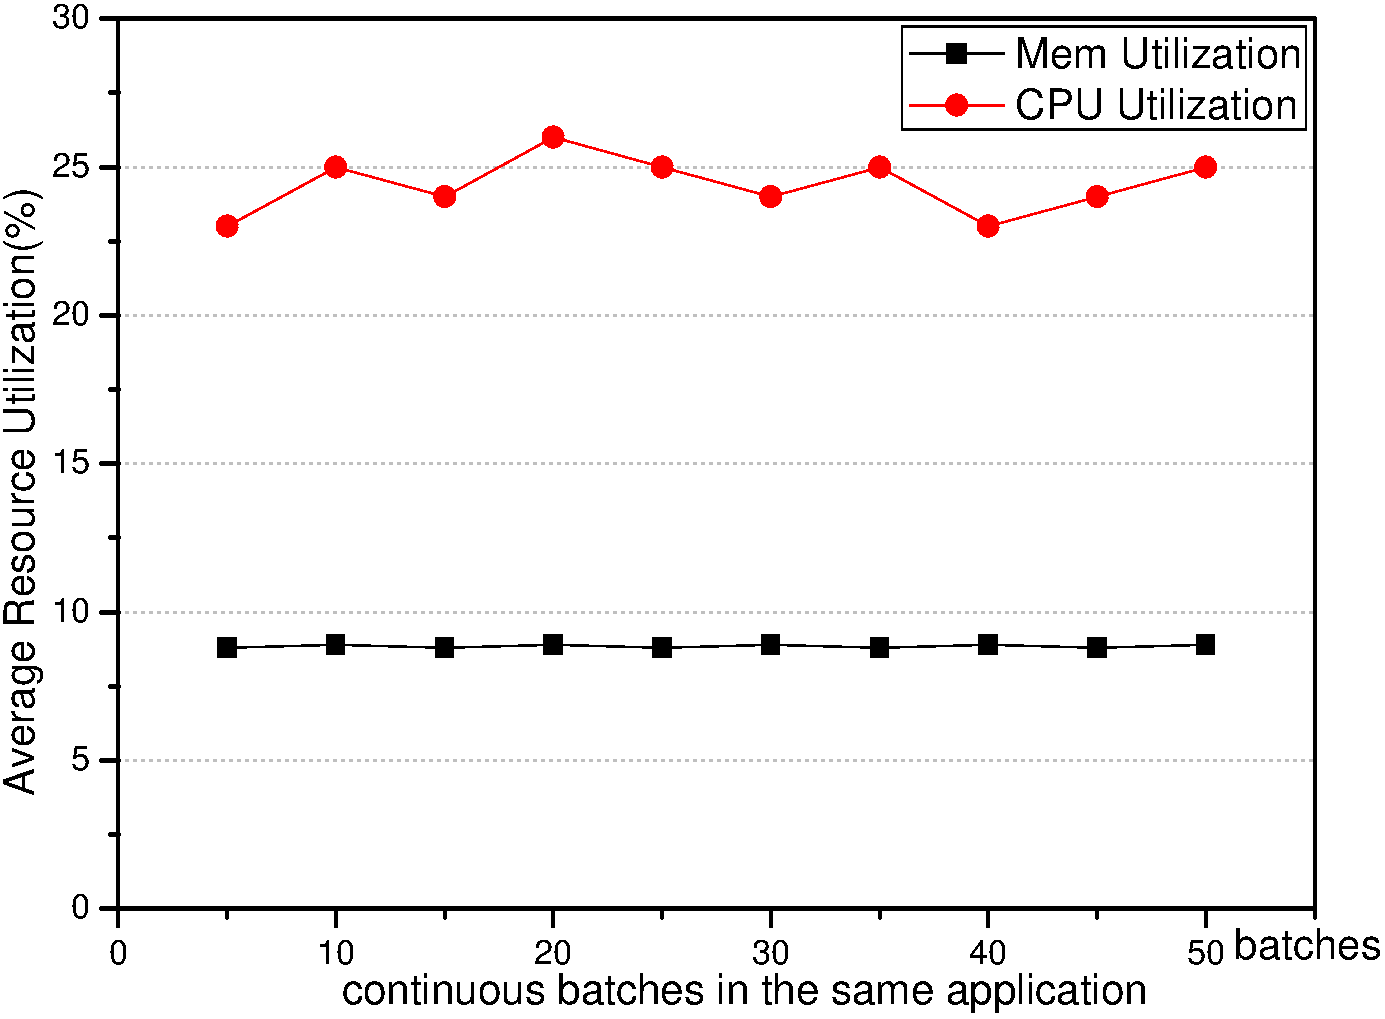
\includegraphics[width=0.24\textwidth]{Figure4}
    }
    \caption{Stability of data properties and resource utilization across recurring jobs when running WordCount}
    \label{Fig. 3:}
  \end{figure}

  Considering the following two points that 1) Straggler characteristics can often be accurately predicted in recurring jobs and 2) Job input data can be assigned in designated locations before scheduling to avoid straggler in advance, We propose Lever, a pre-scheduling straggler mitigation framework that continuously observes and learns the characteristics as recurring jobs execute over time and make a careful assignment about job input data ahead of execution. Doing so, Lever can efficiently reduce the number of queued tasks and avoid stragglers.

\subsection{Challenges}

  We are faced with three challenges:

  Challenge 1 How to identify potential stragglers?

  Before pre-scheduling, Lever need to know which nodes will be stragglers in next batch. Unlike traditional ways which identify stragglers based on runtime-aware decisions, pre-scheduling takes actions before scheduling. Lever leverages the historical information of recurring jobs. But only analyzing historical information is not enough due to the variability of stream load. Accurately identifying potential stragglers is a prerequisite step for eliminating stragglers.

  Challenge 2 How to define and determine node's capability?

  Lever conducts pre-scheduling based on nodes' computational capability. To achieve this goal, it is necessary to define and determine node's capability. Traditional post-scheduling methods have resource utilization view at runtime and can schedule straggler tasks to that node which has free slots. However, in pre-scheduling solutions, it is impossible because we make pre-scheduling decisions before task scheduling. We should define a metric to determine how much data we should pre-schedule to that node. This metric represents to which degree this node will has free slots in future scheduling. So we introduce the notion of node's capability.

  Challenges 3 How to select suitable helpers for data assignment?

  To pre-schedule input data as evenly as possible to eliminate stragglers, Lever need to choose some helpers which are eligible to provide assistance. These helpers should be underloaded and have spare capability in next batch to deal with extra work assigned to them. As explained in Challenge 2, pre-scheduling don't have the perspective of runtime resource utilization. It brings great challenges when we make decisions about which nodes can afford extra load. How to choose suitable helpers with being unaware of task scheduling is a challenging problem.

  \begin{figure}[htbp]
    \centering
    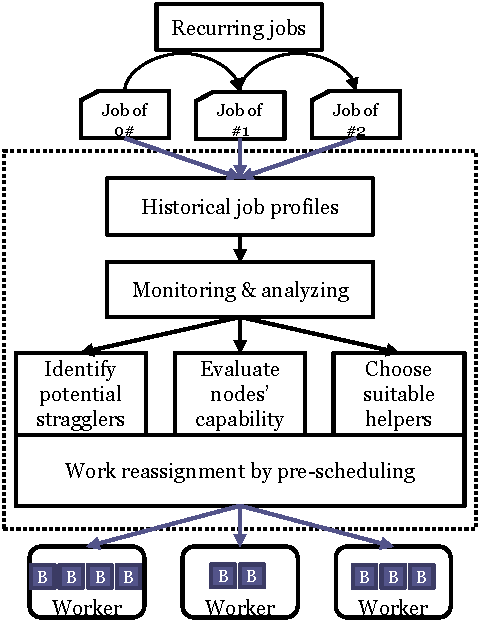
\includegraphics[width=0.35\textwidth]{FigureArchitecture}
    \caption{Architecture of Lever}
    \label{Fig. 4:}
  \end{figure}
  To overcome these challenges, we design and implement a prototype of Lever.
